\documentclass[10pt]{article}
\usepackage{geometry}
\usepackage{amsmath}
\usepackage{amssymb}
\usepackage{graphicx}

\graphicspath{{img/}}

\geometry{a4paper, left=1cm, right=1cm, top=0.5cm, bottom=0.5cm}

\let\olditemize\itemize
\renewcommand\itemize{\olditemize\setlength\itemsep{0em}}
\let\oldenumerate\enumerate
\renewcommand\enumerate{\oldenumerate\setlength\itemsep{0em}}

\title{Esercizi Esame ALAN}
\author{}
\date{}

\begin{document}
\maketitle
\section{Esercizio 1: Errori}
\subsection{Condizionamento}
Calcolare il condizionamento usando l'algoritmo più semplice usando la formula:
\begin{equation*}
    C_{f}=\frac{x(f'(x))}{f(x)}
\end{equation*}
Poi calcolarne il limite:
\begin{itemize}
    \item "Per piccoli valori di $x$" $\rightarrow \lim_{x \to 0}C_{f}$
    \item "Per piccoli valori positivi di $x$" $\rightarrow \lim_{x \to 0^{+}}C_{f}$
    \item "Per grandi valori di $x$" $\rightarrow \lim_{x \to +\infty}C_{f}$
\end{itemize}
Se il limite intorno a $\pm 1$ è ben condizionato, altrimenti è mal condizionato.\\
Il risultato del limite serve per calcolare l'errore inerente:
\begin{equation*}
    Err.Inerente = C_{f}\cdot Err.Input
\end{equation*}
\subsection{Errori negli algoritmi}
Si disegnano i grafi degli algoritmi e l'etichetta degli archi è:
\begin{center}
    \begin{tabular}{|c|c|}
        \hline
        $a\pm b$ & $\varepsilon_{a\pm b}=\frac{a}{a\pm b}\varepsilon_{a}\pm\frac{b}{a\pm b}\varepsilon_{b}$\\
        \hline
        $a\cdot b$ & $\varepsilon_{a\cdot b}=\varepsilon_{b}+\varepsilon_{a}$\\
        \hline
        $\frac{a}{b}$ & $\varepsilon_{\frac{a}{b}}=\varepsilon_{b}-\varepsilon_{a}$\\
        \hline
        $g(x)$ & $\varepsilon_{g(x)}=C_{g(x)}\cdot \varepsilon_{x}$\\
        \hline
    \end{tabular}
\end{center}
Per ogni nodo (a partire dal fondo) si apre una parentesi e dentro si moltiplicano tutti gli archi a partire da quel nodo fino alla fine, se ci sono percorsi alternativi si fa la somma dei percorsi.\begin{equation*}
    \varepsilon\{(I\cdot II\cdot\ldots)+(\ldots)+\ldots\}
\end{equation*}
Per verificare la stabilità dell'algoritmo bisogna fare il limite tendente a $0^{+}$ di tutti gli archi e se viene finito (per tutti gli archi) è stabile, altrimenti è instabile (ne basta uno per verificarlo).
\subsection*{Esempio}
\section{Esercizio 2: Rotazioni/Riflessioni}
\subsection{Rotazioni di Givens}
Si indica una rotazione di Givens con:
\begin{equation*}
    G(i,j,\theta)
\end{equation*}
dove $i$ rappresenta la posizione del perno all'interno della matrice, $j$ la posizione dell'elemento da azzerare e $\theta$ l'angolo di rotazione (che ignoreremo per l'esercizio). Ogni rotazione azzera un elemento ($j$) e cambia il valore del perno $i$ (0 non può essere perno). Si calcola il valore di $c$ e $s$ ad ogni passaggio:
\begin{equation*}
    c = \cos(\theta)=\frac{x_{i}}{\sqrt{x_{i}^{2}+x_{j}^{2}}}
\end{equation*}
\begin{equation*}
    s = \sin(\theta)=\frac{-x_{j}}{\sqrt{x_{i}^{2}+x_{j}^{2}}}
\end{equation*}
Si costruisce la matrice quadrata (della stessa dimensione dei vettori) inserendo $c$ e $s$:
\begin{itemize}
    \item $c$ e $-s$ nella riga $i$
    \item $c$ e $s$ nella riga $j$ 
\end{itemize}
$c$ va nella diagonale, $s$ e $-s$ bisogna posizionarli nella colonna dove c'è l'altro $c$.\\
Si moltiplica la matrice per il vettore iniziale per ottenere il vettore finale/intermedio $\gamma$. Usiamo $\gamma$ per fare un'altra rotazione fino a quando non è uguale al vettore finale.\\
\subsubsection*{Esempio}
\begin{center}
    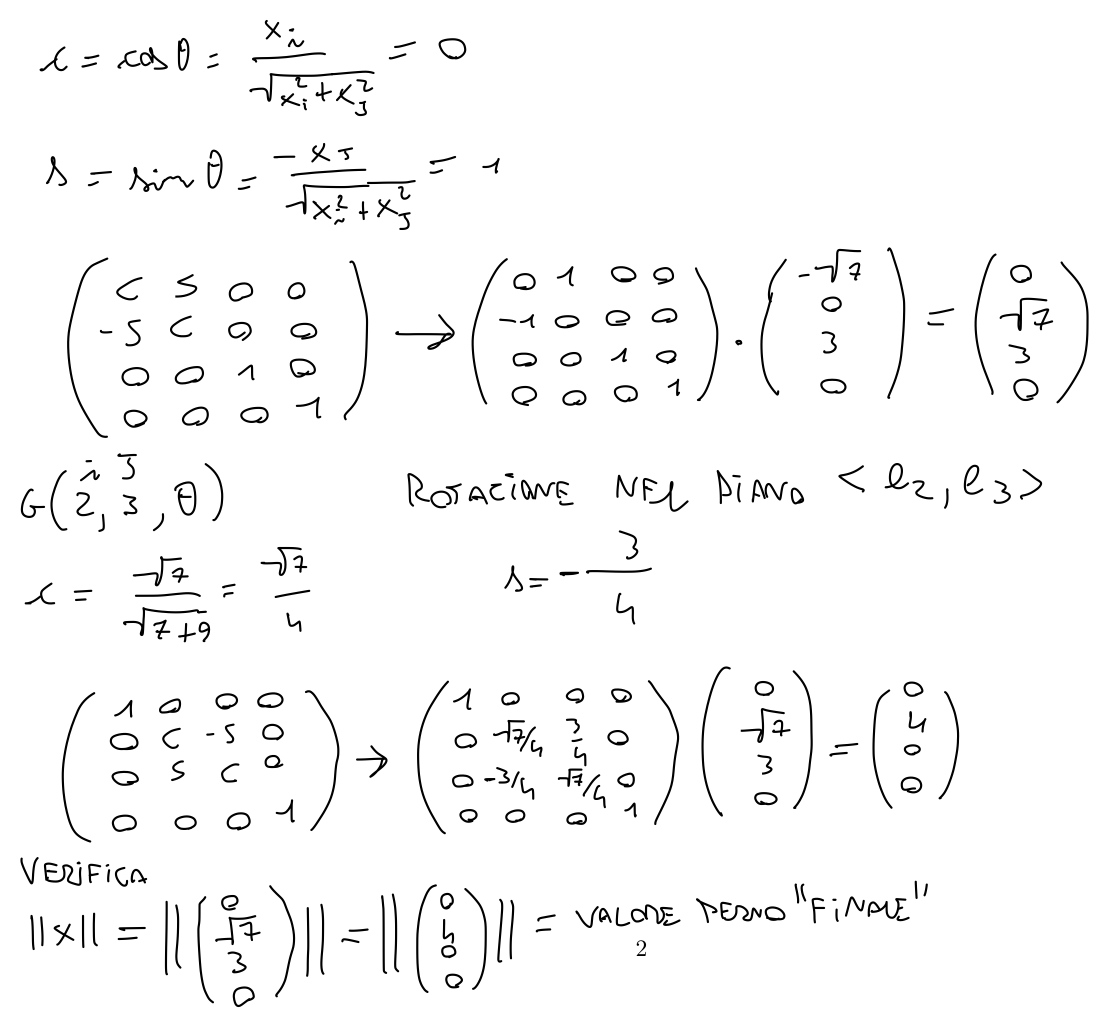
\includegraphics[scale=0.3]{givens.png}
\end{center}
\subsubsection{Interpretazione geometrica}
Per ogni rotazione, scrivere su che piano è stata fatta, ad esempio con la rotazione $G(2,1,\theta)$ si può dire: "si tratta di una rotazione nel piano $<e_{2},e_{1}>$". Visto che sono tutte isometrie: \begin{equation*}
    \lVert \text{vettore iniziale} \rVert = \lVert \text{vettore finale} \rVert
\end{equation*}
Si può usare come prova.
\subsection{Riflessioni di Householder}
\textbf{NB:} abbiamo visto solo come ottenere una riflessione di Householder nel caso in cui $\alpha$ sia il primo elemento del vettore risultante.
\begin{enumerate}
    \item Si calcola $\alpha=\lVert x\rVert_{2}$
    \item Si calcola $u=x-\begin{pmatrix}
        \alpha \\ 0 \\ \vdots \\ 0
    \end{pmatrix}$
    \item Si calcola $u^{T}\bigotimes u \rightarrow \begin{pmatrix}
        x_{1} \\ x_{2}
    \end{pmatrix}\bigotimes\begin{pmatrix}
        y_{1} \\ y_{2}
    \end{pmatrix}=\begin{pmatrix}
        x_{1}\cdot y_{1} & x_{1}\cdot y_{2} \\
        x_{2}\cdot y_{1} & x_{2}\cdot y_{2}
    \end{pmatrix}$
    \item Si crea la matrice (quadrata) identità $I$ con dimensione del vettore $x$ 
    \item Si calcola P: \begin{equation*}
        P = I-\frac{2}{\lVert u\rVert^{2}}\cdot uu^{T}
    \end{equation*}
    \item Infine si calcola $Px$ trovando così il vettore risultante
\end{enumerate}
\subsubsection{Verifiche}
\begin{itemize}
    \item $P$ è ortogonale: colonne perpendicolari, prodotto scalare = 0, colonne normalizzate ($\lVert\text{colonna}\rVert_{2}=1$)
    \item $P\cdot x = \alpha e_{1}$
\end{itemize}
\subsubsection{Interpretazione geometrica}
Si scrive: $P=(\ldots)$ riflette $x=\left(\vdots\right)$ rispetto al piano perpendicolare (al vettore $w$)
\subsubsection*{Esempio}
\begin{center}
    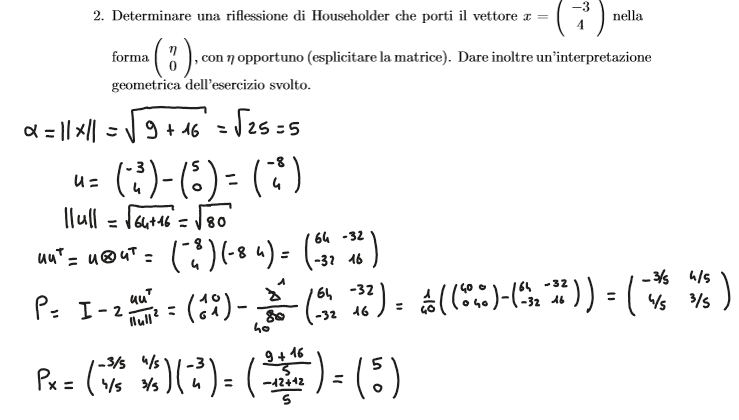
\includegraphics[scale=0.5]{householder.png}
\end{center}
\section*{Esercizio 3: Minimi quadrati}
\begin{equation*}
    f(x) = \alpha g(x)\pm \beta h(x) \pm \ldots \pm \gamma k(x)
\end{equation*}
\begin{tabular}{c | c}
    x & $x_{1}$ $x_{2}$ \ldots $x_{n}$\\
    \hline
    y & $y_{1}$ $y_{2}$ \ldots $y_{n}$
\end{tabular}
\begin{equation*}
    A =
    \begin{pmatrix}
        g(x_{1}) & h(x_{1}) & \ldots & \gamma k(x_{1})\\
        g(x_{2}) & h(x_{2}) & \ldots & \gamma k(x_{2})\\
        \vdots & \vdots & \ddots & \vdots\\
        g(x_{n}) & h(x_{n}) & \ldots & \gamma k(x_{n})
    \end{pmatrix}
\end{equation*}
\begin{itemize}
    \item Se c'è solo la costante senza funzione associata, la sua colonna corrispondente sarà composta solo da 1
    \item Matrice incognite: $A^{T}A$
    \item Matrice soluzioni: $A^{T}\begin{pmatrix}
        y_{1} \\ y_{2} \\ \vdots \\ y_{n}
    \end{pmatrix}$
    \item Usiamo la matrice delle incognite per costruire il sistema (ad esempio $\alpha$ è associata alla prima colonna, $\beta$ alla seconda e così via moltiplicando le incognite con i valori della colonna e sommandoli tra loro) e poniamo ogni riga uguale alla corrispondente riga della matrice soluzioni. Isolo le incognite e poi le sostituisco nella funzione di partenza.
\end{itemize}
\subsection{Interpretazione geometrica}
Disegnare il grafico con i punti e la funzione ricavata, evidenziando le distanze tra i punti dati e il grafico. In più si può scrivere: "la retta di regressione minimizza la somma degli scarti tra i valori di $y$ dei punti ed i valori (equazione del grafico) dell* (nome funzione) calcolat* nelle ascisse $x$ dei punti dati".
\subsection{Esempio}
\begin{center}
    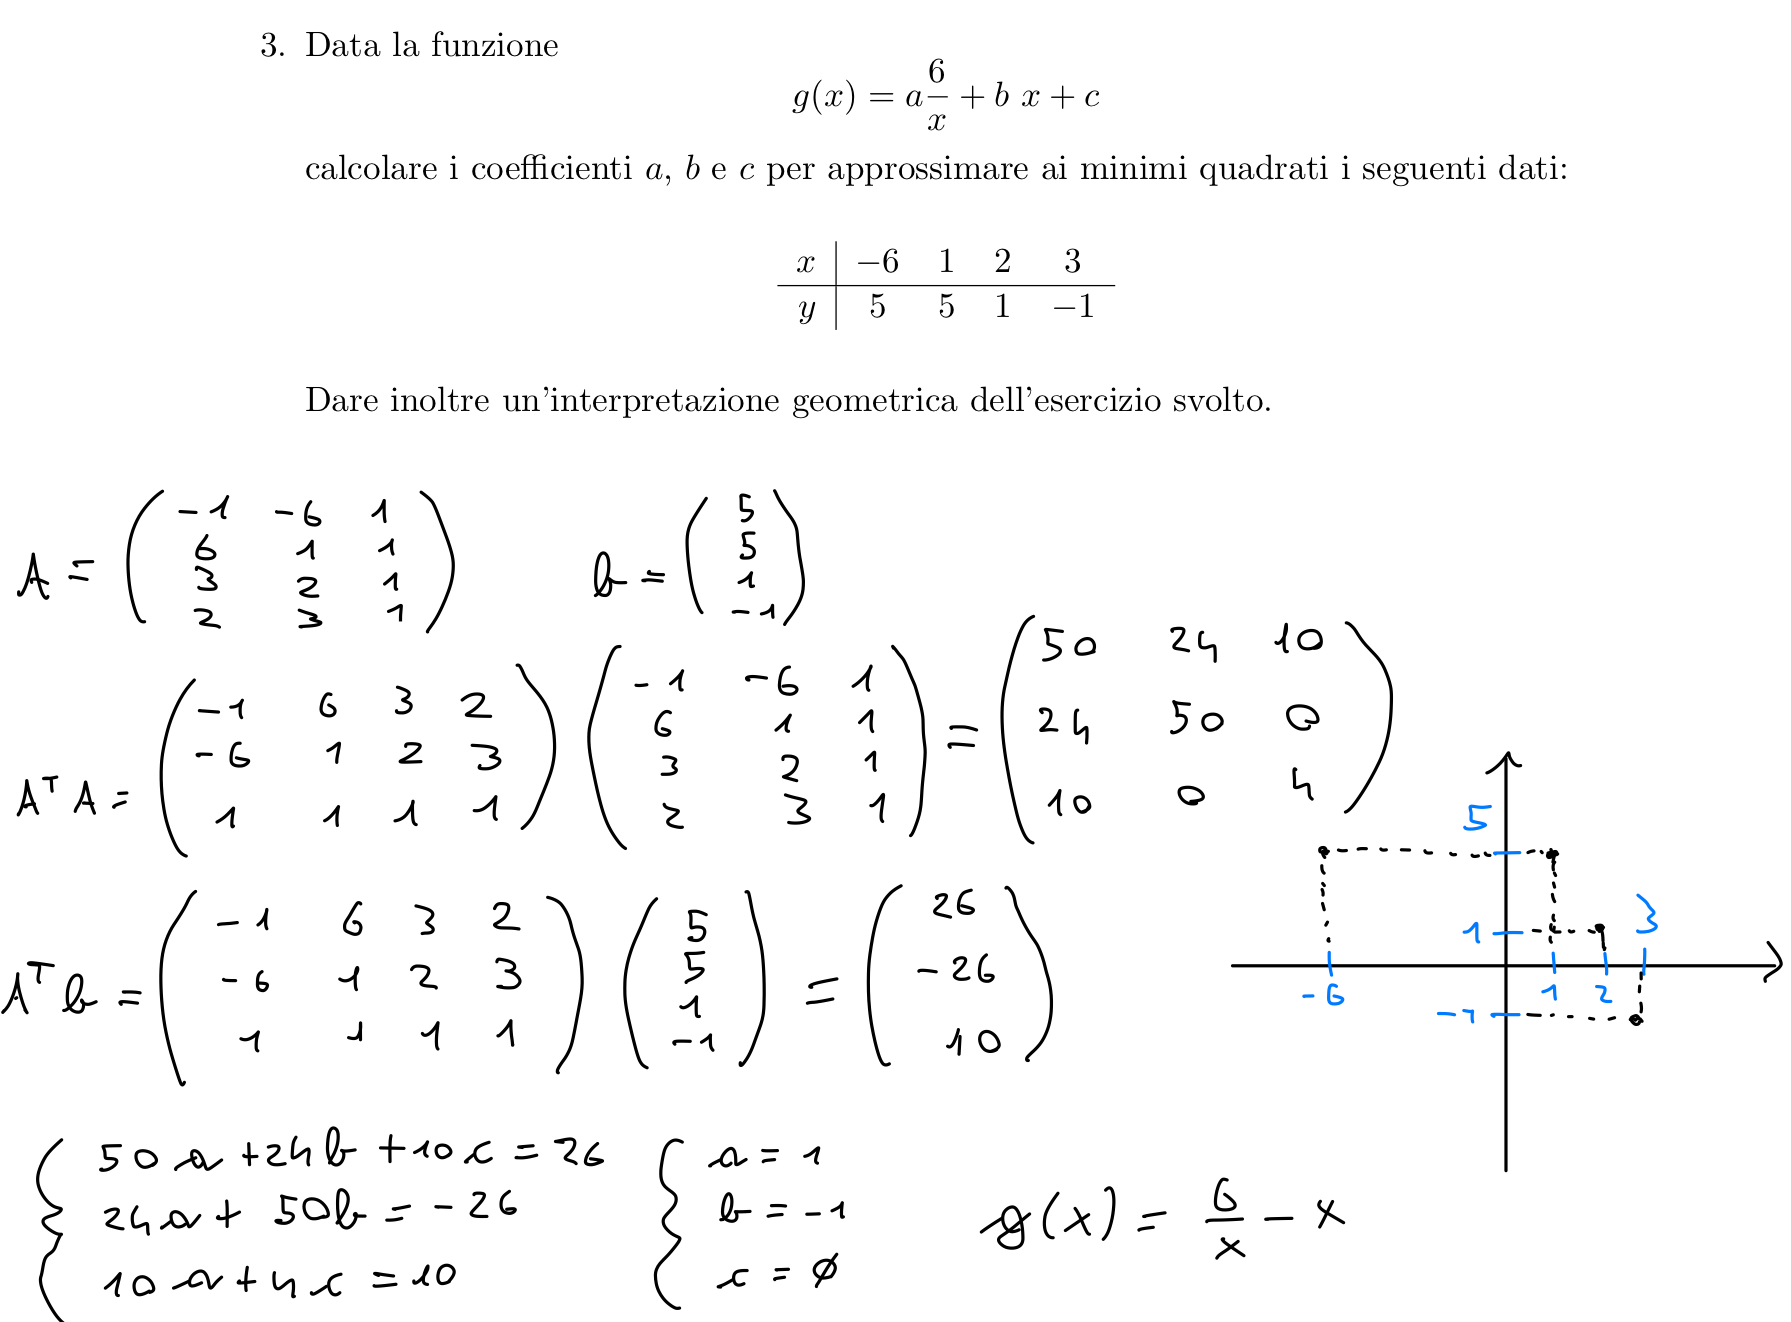
\includegraphics[scale=0.4]{es3pt2.png}
\end{center}
\section*{Esercizio 4: Diagonalizzazione}
\begin{enumerate}
    \item Controllare se $A$ è simmetrica, se lo è, allora è diagonalizzabile
    \item Trovare gli autovalori risolvendo \begin{equation*}
        \det(A-\lambda I)=0
    \end{equation*} e ordinarli in ordine decrescente
    \item Verificare che la quantità di autovalori sia uguale all'ordine della matrice (es. una $2\times 2$ ha ordine 2), altrimenti non è diagonalizzabile
    \item Per ogni autovalore trovare gli autovettori usando la matrice $A-\lambda I$ (sostituendo a $\lambda$ l'autovalore) e risolvendo il sistema \begin{equation*}
        \begin{pmatrix}
            A - \lambda I
        \end{pmatrix}
        \cdot
        \begin{pmatrix}
            x_{1} \\ x_{2} \\ \vdots \\ x_{n}
        \end{pmatrix}
        = \begin{pmatrix}
            0 \\ 0 \\ \vdots \\ 0
        \end{pmatrix}
    \end{equation*}
    \item Normalizzare gli autovettori usando: $\frac{x_{i}}{\lVert v\rVert}$ dove $v$ è l'autovettore e $x_{i}$ è l'elemento $i$-esimo dell'autovettore, controllare se sono indipendenti tra di loro altrimenti non è diagonalizzabile
    \item Creare la matrice $V$ composta dagli autovettori, e la sua inversa
    \item Creare la matrice $D$ usando gli autovalori in ordine decrescente sulla diagonale. $\begin{pmatrix}
        \lambda_{1} & 0 & \ldots & 0\\
        0 & \lambda_{2} & \ldots & 0\\
        \vdots & \vdots & \ddots & \vdots\\
        0 & 0 & \ldots & \lambda_{n}
    \end{pmatrix}$
    \item Si otterrà la diagonalizzazione della matrice di partenza composta nel seguente modo: \begin{equation*}
        A = VDV^{-1}
    \end{equation*}
\end{enumerate}
\subsubsection*{Esempio}
\begin{center}
    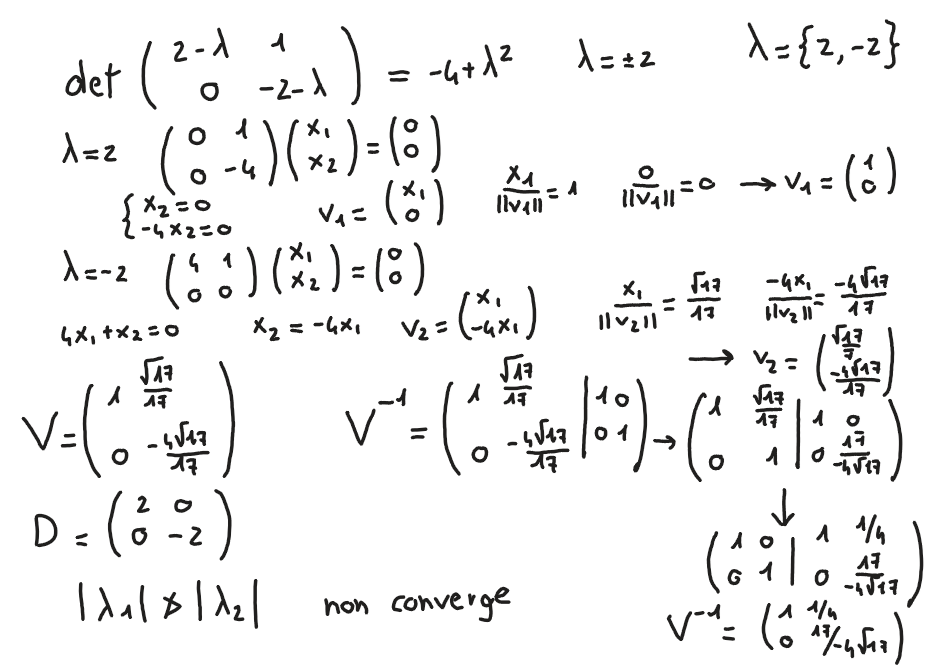
\includegraphics[scale=0.4]{es4pt2.png}
\end{center}
\subsection{Convergenza: Metodo delle potenze}
Converge all'autovalore di massimo modulo
\begin{enumerate}
    \item Si riordinano gli autovalori in base al massimo modulo, ottenendo $\lambda_{1}$, $\lambda_{2}, \ldots, \lambda_{n}$ dove $\lambda_{1}$ è l'autovalore di massimo modulo
    \item Converge se $\lambda_{1}>\lambda_{2}$
    \item $k$ il numero di volte in cui si esegue la moltiplicazione $v_{i} = A\cdot v_{i-1}$, $v_{n}=A\cdot v_{n-1}=A^{2}\cdot v_{n-2} = \ldots = A^{n}\cdot v_{0}$
    \item Si trova la velocità di convergenza con: \begin{equation*}
        V=\left(\frac{\lambda_{2}}{\lambda_{1}}\right)^{k}
    \end{equation*}
\end{enumerate} 
\subsection{Convergenza: Metodo delle potenze inverse}
\begin{enumerate}
    \item Dato uno shift $p$, bisogna trovare l'autovalore più vicino a $p(\lambda_{1})$ ed il secondo più vicino a $p(\lambda_{2})$
    \item Si calcola \begin{equation*}
        \mu_{1} = \frac{1}{\lambda_{1}-p}
    \end{equation*}
    Per ogni $\lambda$
    \item $\mu_{1}$ sarà quello di massimo modulo tra tutti i $\mu$ calcolati, mentre $\mu_{2}$ sarà il secondo di massimo modulo
    \item La velocità di convergenza si calcola: \begin{equation*}
        V = \left(\frac{\mu_{2}}{\mu_{1}}\right)^{k}
    \end{equation*}
\end{enumerate}
Se si hanno due autovalori con lo stesso modulo massimo, allora non converge.
\section{Esercizio 5: Spline}
Si ha una spline se:
\begin{itemize}
    \item $S$ è composta da polinomi di grado $\leq n$, dove $n$ è il grado della spline (ad esempio, una spline di grado 3 sarà composta da soli polinomi di grado $\leq 3$)
    \item $S$ è continua negli estremi interni dei vari intervalli facendo: \begin{equation*}
        \lim_{x\to n^{-}}S(x)=\lim_{x\to n^{+}}S(x)
    \end{equation*}
    \item $S'$ è continua negli estremi interni dei vari intervalli facendo: \begin{equation*}
        \lim_{x\to n^{-}}S'(x)=\lim_{x\to n^{+}}S'(x)
    \end{equation*}
    \item $S''$ è continua negli estremi interni dei vari intervalli facendo: \begin{equation*}
        \lim_{x\to n^{-}}S''(x)=\lim_{x\to n^{+}}S''(x)
    \end{equation*}
\end{itemize}
\subsection{Calcolo dei momenti}
Dato un nodo $K$, si calcola $S''(K)$
\subsection{Periodicità di una spline}
Una spline è periodica se:
\begin{equation*}
    \lim_{x\to e_{1}^{-}}S(x)=\lim_{x\to e_{2}^{+}}S(x)
\end{equation*}
\begin{equation*}
    \lim_{x\to e_{1}^{-}}S'(x)=\lim_{x\to e_{2}^{+}}S'(x)
\end{equation*}
\begin{equation*}
    \lim_{x\to e_{1}^{-}}S''(x)=\lim_{x\to e_{2}^{+}}S''(x)
\end{equation*}
Dove $e_{1}$ e $e_{2}$ sono i due estremi (sinistro e destro rispettivamente) della spline.
\section{Esercizio 5: Condizionamento matrice e di una norma}
Per verificare se la matrice $A^{-1}$ è l'inversa bisogna vedere se $\det(A)\neq 0$ e se $A^{-1}A=I$. Per calcolare il condizionamento relativo ad una norma, bisogna fare:
\begin{equation*}
    \lVert A \rVert_{nm}
\end{equation*}
\begin{equation*}
    \lVert A^{-1} \rVert_{nm}
\end{equation*}
dove $nm$ indica la norma in questione. Poi $M(A)=\lVert A \rVert_{nm}\cdot \lVert A^{-1} \rVert_{nm}$ per calcolare la maggiorazione dell'errore:
\begin{equation*}
    \varepsilon_{x}=\frac{\lVert \bar{x} -x \rVert_{nm}}{\lVert x \rVert_{nm}}
\end{equation*}
\begin{equation*}
    \varepsilon_{b}=\frac{\lVert \delta b \rVert_{nm}}{\lVert b \rVert_{nm}}
\end{equation*}
\begin{equation*}
    \varepsilon_{x}\leq u(A)\varepsilon_{b}
\end{equation*}
Quindi se l'esercizio chiede di calcolare una maggiorazione, basta calcolarsi $u(A)$ e $\varepsilon_{b}$
\subsection{Norme}
\subsubsection{Vettori}
\begin{equation*}
    \lVert x \rVert_{1} = \sum_{i=1}^{n}\lvert x_{i} \rvert
\end{equation*}
\begin{equation*}
    \lVert x \rVert_{2} = \sqrt{\sum_{i=1}^{n}x_{i}^{2}} = \sqrt{x^{T}x}
\end{equation*}
\begin{equation*}
    \lVert x \rVert_{\infty} = \max_{1\leq i\leq n}\lvert x_{i} \rvert
\end{equation*}
\subsubsection{Matrici}
\begin{equation*}
    \lVert A \rVert_{1} = \max_{1\leq j\leq n}\sum_{i=1}^{n}\lvert a_{ij} \rvert
\end{equation*} (Somma di tutti gli elementi in modulo di una colonna e prendo il massimo)
\begin{equation*}
    \lVert A \rVert_{2}
\end{equation*} Esiste ma non calcolabile esplicitamente
\begin{equation*}
    \lVert A \rVert_{\infty} = \max_{1\leq i\leq n}\sum_{j=1}^{n}\lvert a_{ij} \rvert
\end{equation*} (Somma di tutti gli elementi in modulo di una riga e prendo il massimo)
\section{Esercizio 5: SVD}
Una SVD viene utilizzata per trovare una diagonalizzazione di una matrice non simmetrica scritta nella forma \begin{equation*}
    A = U\Sigma V^{T}
\end{equation*}
\begin{itemize}
    \item $U$ è una matrice ortogonale (ovvero $U^{T}U=UU^{T}=I$)
    \item $\Sigma$ è una matrice diagonale con i valori singolari sulla diagonale in ordine decrescente
    \item $V$ è una matrice ortogonale (ovvero $V^{T}V=VV^{T}=I$)
\end{itemize}
\subsection{Proprietà}
Data una matrice $A\in R^{m\times n}$\\
Immagine: trovare il valore singolare $r$-esimo, ovvero il più piccolo elemento strrettamente maggiore di 0. Per trovare l'immagine scriveremo tutti i vettori $u$ da 1 a $r$: \begin{equation*}
    R(A) = <u_{1}, u_{2}, \ldots, u_{r}>
\end{equation*}
Nucleo: indichiamo con $v$ i vettori che lo compongono, partiranno da $r+1$ fino a $n$:
\begin{equation*}
    N(A)=<v_{r+1}, v_{r+2}, \ldots, v_{n}>
\end{equation*}
Certi esercizi potrebbero chiedere di determinare i valori singolari delle matrici $A^{T}A, AA^{T}, A^{T}$: esistono proprietà specifiche per questi casi.
\subsection{Pseudoinversa}
Dimensione: $\forall A \in \mathbb{R}^{m\times n}: \exists A^{T}\in \mathbb{R}^{m\times n}$
\end{document} 